
\subsection{LHC chamber with sawtooth structure}
The transverse geometry of the LHC chamber is pictured in Fig.~\ref{fig:beam_screen_structure}.
Of great importance is the sawtooth structure that ensures an almost normal impact of most photons on the surface, which greatly reduces the reflectivity.
Therefore, most photoelectrons are created at the outer part of the beam screens, where they do not significantly contribute to the electron cloud buildup.

\begin{figure}[tbh]
    \centering
    \begin{minipage}[c]{0.47\textwidth}
        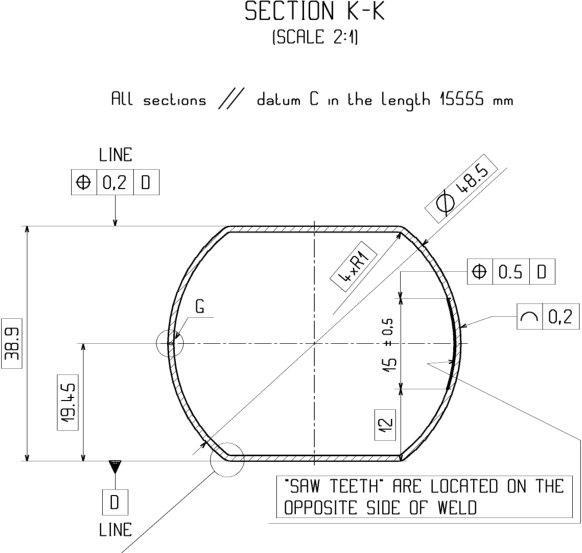
\includegraphics[width=\textwidth]{../ss/beam_screen_drawing.png}
    \end{minipage}
    \hspace{0.5cm}
    \begin{minipage}[c]{0.47\textwidth}
        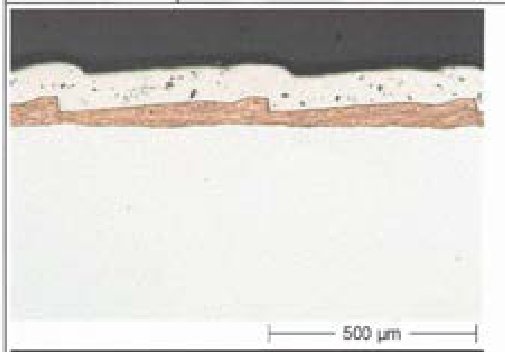
\includegraphics[width=\textwidth]{../ss/sawtooth_fine.png}
    \end{minipage}
\caption{
        Left: the technical drawing of the LHC beam screen~\cite{beam_screen_drawing}. Right: a closeup of the sawtooth structure. The vertical edges are about 35~$\mu$m long~\cite{zimmermann}.
        }
\label{fig:beam_screen_structure}
\end{figure}

\subsection{Simulated electron stripes in LHC magnets}

\begin{figure}[tbh]
    \centering
    \begin{minipage}[c]{0.47\textwidth}
        \includegraphics[width=\textwidth]{../ss/Pass00050_00004.png}
    \end{minipage}
    \hspace{0.5cm}
    \begin{minipage}[c]{0.47\textwidth}
        \includegraphics[width=\textwidth]{../ss/pass_oct.png}
    \end{minipage}
    \caption{Simulated electron densities for a dipole and an octupole.}
    \label{fig:sim_densities}
\end{figure}

\subsection{SynRad3D simulations}
The azimuthal distributions of absorbed photons in the LHC chamber have been simulated with the code SynRad3D~\cite{guillermo}.
The photons origin from a beam with 7~TeV energy, and only photons with more than 4~eV energy are considered.
The results are shown in Fig.~\ref{fig:guillermo}.
With access to the raw data, it could be converted to the PyECLOUD input parameter \textbf{inv\_CDF\_refl\_photoem\_file}.

The comparison with several cosine curves in Fig.~\ref{fig:guillermo} shows that the simulated distributions is much narrower than practically any cosine distribution.
The distribution of electrons in a dipole is concentrated in stripes which range from MISSING PIC.
This leads to much higher photoelectrons at angles of 90$^\circ$, where they are most relevant to the buildup process.

\begin{figure}[tbh]
    \centering
    \begin{minipage}[c]{0.47\textwidth}
        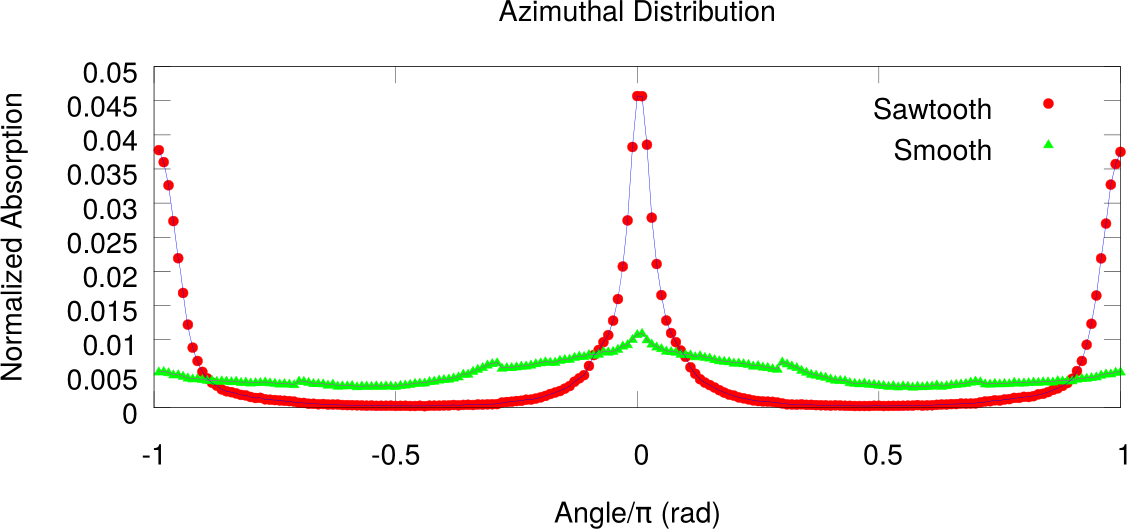
\includegraphics[width=\textwidth]{../ss/photon_distribution_guillermo.png}
    \end{minipage}
    \hspace{0.5cm}
    \begin{minipage}[c]{0.47\textwidth}
        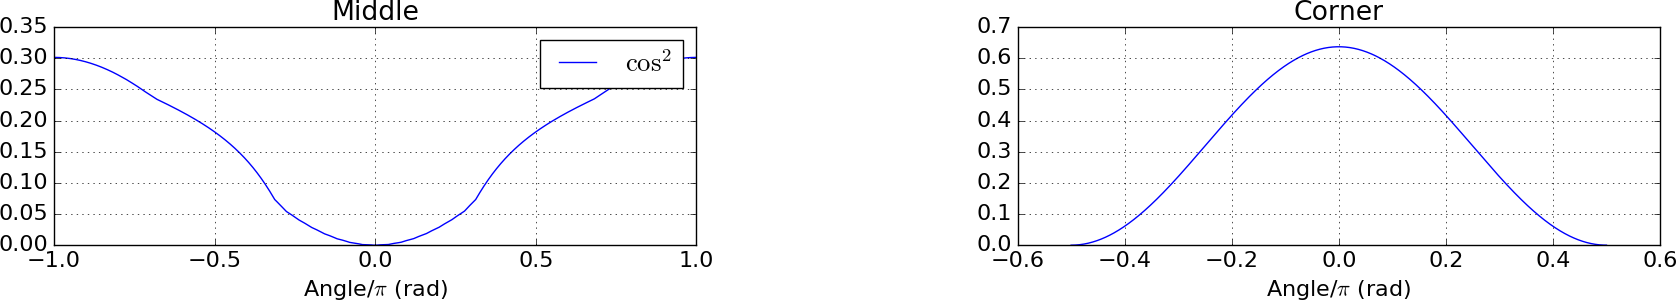
\includegraphics[width=\textwidth]{../plots/cosine_power.png}
    \end{minipage}
    \caption{Left: The photon distribution as it was simulated for the LHC chamber geometry with and without sawtooth~\cite{guillermo}.
    An angle of 0 corresponds to the impact point of the synchrotron radiation.
    Right: Several powers of cosine distributions for a comparison.}
    \label{fig:guillermo}
\end{figure}

\subsection{SynRad+ simulations}

The SynRad+ tool has been developed at CERN~\cite{synrad+}, and is being used for simulations of future machines.
Results concerning the current LHC have not been published.
However simulations for the sawtooth structure have been performed, see Fig.~\ref{fig:synrad}.
These look very promising and could lead to very useful information concerning electron-cloud simulations.

\begin{figure}[tbh]
    \centering
    \begin{minipage}[t]{0.47\textwidth}
        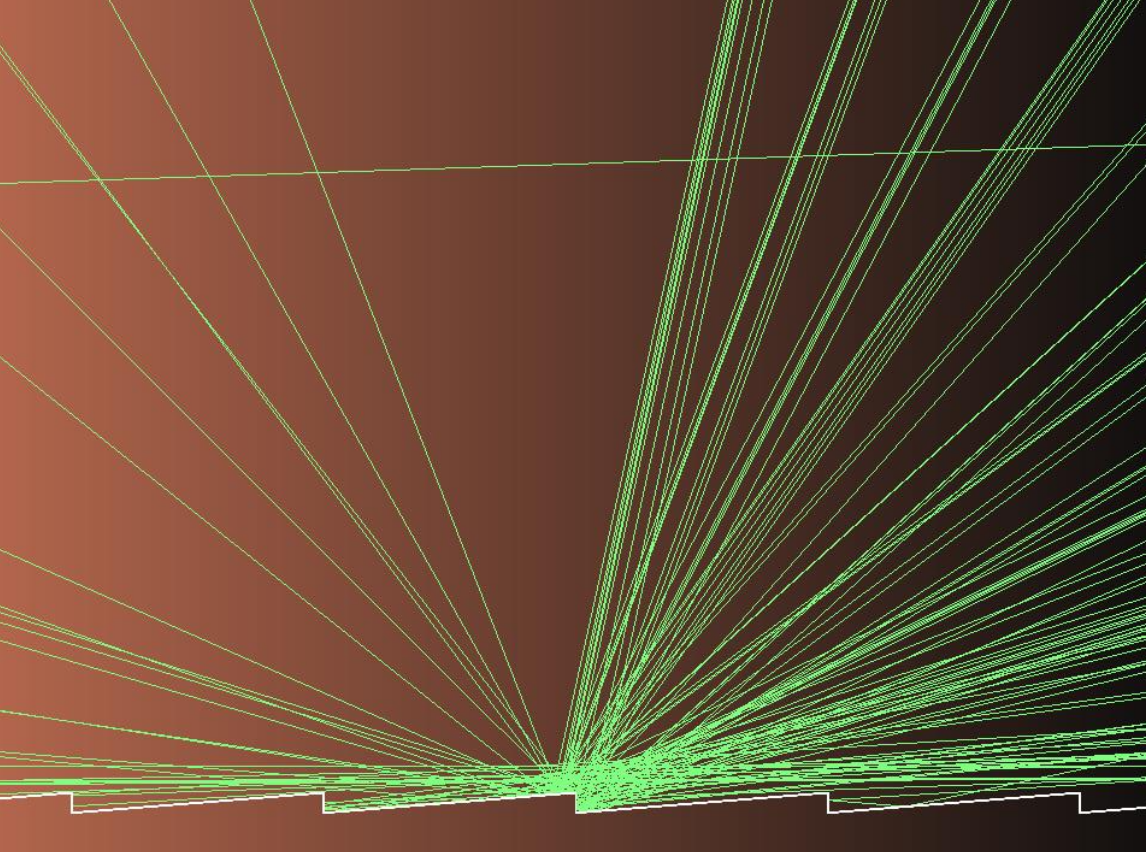
\includegraphics[width=\textwidth]{../ss/synrad_plus_sawtooth.png}
    \end{minipage}
    \hspace{0.5cm}
    \begin{minipage}[t]{0.47\textwidth}
        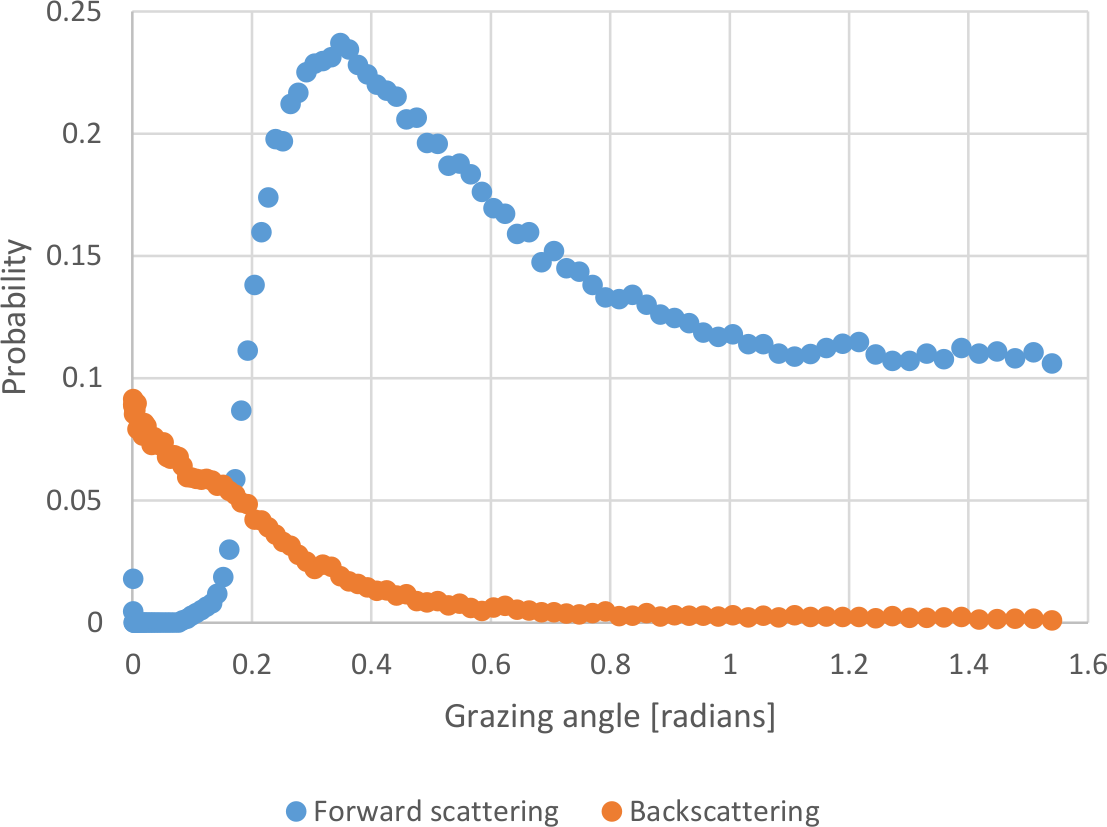
\includegraphics[width=\textwidth]{../ss/synrad_plus_sawtooth_refl.png}
    \end{minipage}
    \caption{
        Left: simulated photon reflections from the sawtooth surface with SynRad+.
        \\
        Right: Extracted reflection probabilities from the sawtooth simulations for 10~eV photons~\cite{synrad+}.
    }
    \label{fig:synrad}
\end{figure}

